%%%%%%%%%%%%%%%%%%%%%%%%%%%%%%%%%%%%%%%%%
% This document provides a sample senior 
% thesis proposal template for use
% by Allegheny's Computer Science majors.
%
% This template was adopted from Jeremie Gillet
% Ref: https://github.com/oist/LaTeX-templates
%
% Author: Janyl Jumadinova
% Last Updated: November 5, 2019
%
%%%%%%%%%%%%%%%%%%%%%%%%%%%%%%%%%%%%%%%%%

%----------------------------------------------------------------------------------------
%	PACKAGES AND OTHER DOCUMENT CONFIGURATIONS
%----------------------------------------------------------------------------------------

\documentclass[12pt,oneside]{book} % 12 pt font, one-sided book style
\usepackage[a4paper, includehead, headheight=0.6cm, inner=3cm ,outer=2.5cm, top=2.5 cm, bottom=2.5cm]{geometry}  % Changing size of document
\usepackage[english]{babel} % The document is in English
\usepackage[utf8]{inputenc} % UTF8 encoding
\usepackage[T1]{fontenc} % Font encoding

\usepackage{graphicx} % For including images
\graphicspath{{./images/}} % Specifies the directory where images are stored

\usepackage{longtable} % tables that can span several pages
\usepackage[bf]{caption} % caption: FIG in bold
\usepackage{fancyhdr} % For the headers

\newcommand{\numberedchapter}{ % Preparation for numbered chapters
	\cleardoublepage % To make sure the previous headers are passed
	\fancyhead[RE]{{\bfseries \leftmark}}% Headers for left pages
	\fancyhead[LO]{{\bfseries \rightmark}}}% Headers for right pages
\newcommand{\unnumberedchapter}[1]{ % Preparation for unnumbered chapters
	\cleardoublepage % To make sure the previous headers are passed
	\addcontentsline{toc}{chapter}{#1} % Also adds the chapter name to the Contents
	\fancyhead[RE]{{\bfseries #1}} % Headers for left pages
	\fancyhead[LO]{}}%Headers for right pages

\usepackage{emptypage} % No headers on an empty page

\usepackage{eso-pic} % For the background picture on the title page
\newcommand\BackgroundPic{%
\put(0,-120){%
\parbox[b][\paperheight]{\paperwidth}{%
\vfill
\centering

\includegraphics[width=4in]{images/logo}%
\vfill
}}}

\usepackage{hyperref} % Adds clickable links at references

%----------------------------------------------------------------------------------------
%	ADD YOUR CUSTOM VALUES, COMMANDS AND PACKAGES
%----------------------------------------------------------------------------------------

% Open preamble/mydefinitions.tex and enter some values (name, thesis title...) 
% and include your own custom LaTeX functions and packages

%----------------------------------------------------------------------------------------
% values for the proposal
%----------------------------------------------------------------------------------------

\newcommand{\name}{Xingbang Liu} % Author name
\newcommand{\thesistitle}{Music Recommendation by Mapping Music and Descriptive Paragraph} % Title of the thesis
\newcommand{\submissiondate}{\today} % Submission date "Month, date year"
\newcommand{\supervisor}{Janyl Jumadinova} % First reader's name
\newcommand{\cosupervisor}{Gregory M. Kapfhammer} % Second reader's name


%----------------------------------------------------------------------------------------
%	BIBLIOGRAPHY STYLE
%----------------------------------------------------------------------------------------


\bibliographystyle{acm}

%----------------------------------------------------------------------------------------
%	YOUR PACKAGES (be careful of package interaction)
%----------------------------------------------------------------------------------------

\usepackage{amsthm,amsmath,amssymb,amsfonts,bbm}% Math symbols

%----------------------------------------------------------------------------------------
%	YOUR DEFINITIONS AND COMMANDS
%----------------------------------------------------------------------------------------

% New Commands
\newcommand{\bea}{\begin{eqnarray}} % Shortcut for equation arrays
\newcommand{\eea}{\end{eqnarray}}
\newcommand{\e}[1]{\times 10^{#1}}  % Powers of 10 notation


\begin{document}

%----------------------------------------------------------------------------------------
%	TITLE PAGE
%----------------------------------------------------------------------------------------

\pagestyle{empty} % No page numbers
\frontmatter % Use roman page numbering style (i, ii, iii, iv...) for the preamble pages

\begin{titlepage}
\AddToShipoutPicture*{\BackgroundPic}
\begin{center}
\vfill
{\large \scshape Allegheny College \\ Department of Computer Science }\\[1.4cm]
{\Large Senior Thesis}\\[0.5cm]
\rule{\textwidth}{1.5pt}\\[0cm]
{\huge \bfseries \thesistitle \par \ }\\[-0.5cm]
\rule{\textwidth}{1.5pt}\\[2.5cm]
\hfill  by\\[1cm]
\hfill  {\large \bfseries\name}\\
\vfill
{\hfill \large Project Supervisor: \textbf{\supervisor}} \\ 
\ifx\cosupervisor\undefined\else{\hfill \large Co-Supervisor: \textbf{\cosupervisor}} \\ \fi
\vspace{1cm}
\hfill  \submissiondate
\end{center}
\end{titlepage}


\pagestyle{fancy} % Changes the headers
\fancyhf{}% Clears header and footer
\fancyhead[RO,LE]{\thepage} % page number on the outside of headers

%-------------------------------------------------------------------------------
%	PREAMBLE PAGES (delete unnecessary pages)
%   preamble pages besides abstract are optional
%-------------------------------------------------------------------------------

\unnumberedchapter{Abstract} 
\chapter*{Abstract} 

Provide a concise summary of your  research project of approximately 250 words. 
Remember that the abstract is {\it not\/} an introduction, it is a {\it summary\/} of the entire document, including the results and future direction of the project.
\unnumberedchapter{Acknowledgment} 
\chapter*{Acknowledgment} 

Theses should acknowledge assistance received in any of the following areas:

\begin{itemize}
\item Designing the research
\item Executing the research
\item Analyzing the data
\item Interpreting the data/research
\item Writing, proofing, or copyediting the manuscript 
\end{itemize}

\unnumberedchapter{Abbreviations} 
\chapter*{Abbreviations} 

All abbreviations used in the thesis should be listed here, with their definitions, in alphabetical order.  This includes trivial and commonly used abbreviations (at your own discretion), but not words that have entered into general English usage (such as laser or DNA).  In particular, non-standard abbreviations should be presented here.  This is an aid to the reader who may not read all sections of the thesis. \\ % You can delete this paragraph, only the table is needed.

\begin{longtable}{rl}
PPT & positive partial transpose\\
SRPT & Schr\"odinger-Robertson partial transpose
\end{longtable}
\unnumberedchapter{Glossary} 
\chapter*{Glossary} 

% Break up this table into several ones if it takes up more than one page
\begin{center}
\begin{longtable}{r p{0.58 \textwidth}}
Dipole Blockade & Phenomenon in which the simultaneous excitation of two atoms is inhibited by their dipolar interaction. \\
Cavity Induced Transparency & Phenomenon in which a cavity containing two atoms excited with light at a frequency halfway between the atomic frequencies contains the number of photons an empty cavity would contain.  \\ 
\end{longtable}
\end{center}

\cleardoublepage
\thispagestyle{empty} % Page style needs to be empty for this page

\vspace*{8cm} 

\hfill
\begin{parbox}{0.6\textwidth}{
\begin{flushright}

If desired, an optional and short dedication may be included here.

\end{flushright}}
\end{parbox}




%-------------------------------------------------------------------------------
%	LIST OF CONTENTS/FIGURES/TABLES
%-------------------------------------------------------------------------------

\unnumberedchapter{Contents}
\tableofcontents % Write out the Table of Contents
\unnumberedchapter{List of Figures}
\listoffigures % Write out the List of Figures
\unnumberedchapter{List of Tables}
\listoftables % Write out the List of Tables

%-------------------------------------------------------------------------------
%	THESIS MAIN TEXT
%-------------------------------------------------------------------------------

\addtocontents{toc}{\vspace{2em}} % Add a gap in the Contents, for aesthetics
\mainmatter % Begin numeric (1,2,3...) page numbering

%----------------------------------------------------------------------------------------
%	START DELETE TEXT
%----------------------------------------------------------------------------------------

\section*{Template Overview}

You should first modify the documents in the preamble, things that appear before the main text as detailed below. 

\textbf{Front page}: use the one provided in this template, after changing the values like names in the file \texttt{preamble/mydefinitions.tex}.

\textbf{Abstract}: There should be a single paragraph of about 250 words, which concisely summarizes the entire proposal, written in the file \texttt{preamble/abstract.tex}.

\textbf{Acknowledgments, Abbreviations, Glossary, Dedication} preamble pages are optional and can be used at the author's discretion. 

The main text of the proposal should be stored in the ``SeniorThesis.tex'' document. The following descriptions are sections that must be included in the thesis document.

\textbf{Bibliography}: The bibliography should include all references cited in the text (as \cite{dasgupta2015comrade}) and it should not include references that have not been cited. ACM referencing style should be used when preparing the bibliography. We recommend using BibTeX or BibLaTeX and using the file \texttt{preamble/bibliography.bib}.

%----------------------------------------------------------------------------------------
% STOP DELETE
%----------------------------------------------------------------------------------------

%\numberedchapter{Introduction} % Title of the numbered chapter
\chapter{Introduction}
\label{ch:intro}

\section{Motivation}
\label{sec:motivation}

It is normal to have the situation that, when people cannot find the right music track for certain emotional states.

\subsection{Human Emotion and Music Emotion}

Humans like music for its capability to express emotions. The study has shown that music can evoke human emotions and influence human moods \cite{Przybysz2013}. In the experiments mentioned by Przybysz, some sad or happy music can cause human physical reactions such as muscle tension and hormone release. This is one of the reasons for the human to have certain emotions toward music. However, sometimes music emotion and human emotion are separate. Human and music may carry the same emotion, for example, sadness, but human sadness and music sadness may be different. The human may be seeking for temporary separation from the real world. Context outside of music could also arouse human emotions. For example, when people are at the funeral, they are meant to be sad. When the lyrics or the music title are sad, people would also feel sad.

As music is so important to humanity and the internet became the most important tool in society nowadays, music service companies started to provide people access to music content and convenient service bundles. Based on different user demands, different music services have different strategies. For example, some users want to access a large number of music tracks with a low cost, some users want to discover new music content in a smart way \cite{palaniappan2018}. Therefore, Spotify provides music stream services, and users have the option to upgrade to Spotify premium. With Spotify premium, users can skip songs, make tracks offline with users options, and more. With a good music service, users use music playlist published by other users to play at coffee shops, users listen to music when exercising, and users play music at weddings.

\subsection{Easy Music Discover}

With a large amount of music content users can access, it would be hard for users to pick the right song at the right moment, expand their playlists, or listen back to the song they saved previously \cite{palaniappan2018}. Therefore, some music service providers developed music recommendation systems for users to find music content smartly. Spotify's Weekly Discovery is a good example for users to expand their playlist based on the music they saved previously. Generally speaking, the music recommendation system we can find on market works in two ways. The first way if to find new music content based on users' previous interested music. The second way is to find users who have similar actions and music preferences and cross recommend songs to each other. Since different users would not possibly have the same music playlist, it would be efficient to suggest new songs to different users.

These music recommendation services are accurate, users may enjoy it, but this system has a limitation. It only digs deeper for user interests, but it does not expand them. The reason is that the information for music recommender systems to use only contains user interaction toward music tracks. The system can classify and rank music tracks that people like or dislike, but they cannot get information about the user's emotional state.

\subsection{User Current Emotion State}

As mentioned before, the relationship between music emotions and human emotions are complicated. Not only some music can evoke human emotions, in some situations, but human emotions can also be evoked by the surroundings, lyrics, and humans may have their emotions and they are seeking similar emotions in music. In situations when people are sad, they want some corresponding sad music tracks to help them relieve mental painfulness. The recommendation system will recommend a list of songs based on user previously saved music. However, users would not only have sad music in their playlist, but they also have happy music. It would be hard for users to locate the songs they want. Although some music services have a sad music classification, users still have to explore more for the music that they want, because the scene defined by the lyrics may be different.

The important part here is to recognize the emotional state of the users. If music service recommends music content based on user current emotion state, the result would be more accurate in terms of user current demand. Therefore, it is better to let users express themselves. Let users define their emotions states themselves. This way, users can get music recommendations more accurate because users know their requirements the best. This solution can also provide a wider range of recommendations because it does not depend on user interaction history. Every music content suggested by this theory would be potentially new from users' past preferences.

\section{Current State of the Art}
\label{sec:stateofart}

There are various music services, such as Spotify, Amazon Prime Music, Pandora, and YouTube Music, that people like to use. The most popular music service on the market would be Spotify. According to MIDiA \cite{midiaresearch}, a company analyzes media and technology, Spotify owns 83 million subscribers and 36\% of the market share \cite{mulligan2018} at H1 of 2018.

\subsection{Spotify}

Spotify has different clients on different platforms. For example, there are mobile clients, desktop clients, TV clients, Web player, and more. Users can choose freely between different platforms. In each Spotify platform, the user can choose their preferred music content to play \cite{Zhang2013}. With smart home technologies got more and more popular, Spotify added functions that can control playback devices on different platforms. For example, users can control Google Home to play music from Spotify by smartphones. Besides the basic music player function, users can also add other users as friends to get other people's music content.

Spotify also has a strong music recommendation system to help people get more new music that they like. Users can get recommendations from Discover Weekly, Daily Remix, and song radios. There are three main techniques Spotify used to get recommendations for the users, which are Collaborative Filtering, Natural Language Processing, and Audio Metadata Modeling. In other words, Spotify utilized information from user interactive history and compares across different users, lyrics semantics, music patterns, and audio metadata, to get similar music contents.

\subsection{YouTube Music}

YouTube Music is another popular music service on the internet nowadays. YouTube was famous for its video services. YouTube users can upload videos they produced. Users who want to enjoy personalized services have to register user accounts. Based on user interests, YouTube would recommend videos on their homepage, and under each video that been played by the users, several related videos would be shown for users to pick. Under each video, users can write comments to share their thoughts. Video providers can also interact with other users. Video producer not only can gain popularity on YouTube but also money from YouTube because YouTube let companies put advertisements in the video contents. This is one of the reasons people are willing to upload videos to YouTube.

YouTube got more and more popular in recent years, they have announced that they have 100 hours of videos uploaded to them every hour in the past \cite{Liikkanen2015}. According to a user insight report in 2018, about 47\% of users listen to music on-demand at Youtube \cite{ifpi}. With such a good user foundation, music producers and companies started to release music videos on YouTube. Based on a large number of licensed music videos, YouTube started music streaming services. With a good video recommendation system, YouTube combined content recommendation and social media functions. Similar users are easier to get each other's suggestions.

\subsection{Netease Cloud Music}

Netease Cloud Music is a Chinese music service provider. Most of the music license is held by Tencent Music at the time. As a new music service provider, to compete with Tencent Music, Netease Cloud Music developed stratify to develop strong music recommendation systems and social media platforms.

They think the essence of music service is to help users find the music they like efficiently. When users find the music they like, they would usually want to express themselves. Therefore, Netease Cloud Music provides comment sections for users to write their feelings and stories. Users can also share music between friends and other social media platforms. Because of the lack of music license, Netease Cloud Music encourages small and new producers to upload music to their platform. They also depend more on music recommendation between similar users. Due to Netease Cloud Music's good reputation among users, they got a great number of fundings recently \cite{russell2018}.

\section{Goals of the Project}
\label{sec:goals}

A new system was proposed to match descriptive paragraphs with music tracks. This way, users can express their emotions whenever it is necessary, and a complex mechanism to detect the user's current emotion state can be avoided. Besides simple emotion detects, they can also expand their music interest by exploring more random but relevant music contents.

\subsection{Scenes}

Multiple scenes would be fit for the project. For example, a person breaks up with his or her girlfriend or boyfriend would be very sad at the moment. People would listen to sad songs when that happens. To find the right music tracks to identify their exact feelings, the person who is experiencing negative emotions can write literature paragraphs. These paragraphs would contain the sentiment of that person, and the story behind the negative emotions. It would be the same for people experiencing positive emotions, such as fall in love with someone.

The scene does not limit to self-generated emotions. For example, a person who watches a film or television could find himself or herself related to the work. The person would listen to related music tracks to express appreciation. Or the filmmakers want to find relevant music that matches the scene of the film, even contains matching metaphor. They can use a description of the film or the film scripts as the descriptive paragraph. By mapping the key factors of the paragraph with the music key factors, the relevant music tracks would be identified.

\subsection{General Workflow}

Before the user uses the service, pre-processing is required to get extra music contexts. The lyrics of the music track would be analyzed, and they would be summarized into keywords. And the result would be stored at the server database.

After the pre-processing is done, this system would firstly take user inputs. However, users are lazy, it always requires more to motivate people to generate sufficient inputs. Therefore, the format of the input has to be closely related to potential emotion breakouts. These inputs can be a diary, personal blog, video script, or description of the video content.

After getting a sufficient amount of user inputs, the system would analyze the inputs, breaks them down into pieces and summarize them into keywords. The sentiment of the text would also be analyzed. This extracted information would be used to compare with the language model in the music dataset. Specifically, the similarity would be checked between user description summarization and music fingerprints.

Finally, the system will return a list of relevant songs to users. The general workflow of the system shown as figure \ref{workflowg}.

\begin{figure}[htbp]
\centering
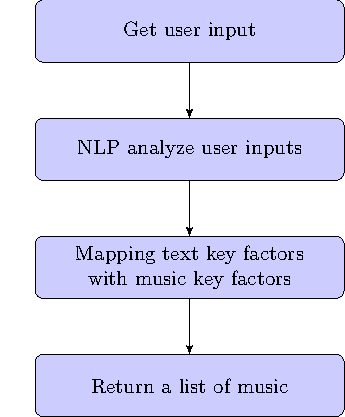
\includegraphics[width=4 in]{images/workflowg}
\caption{General Workflow}
\label{workflowg}
\end{figure}

\section{Thesis Outline}
\label{sec:outline}

In this project paper, five sections will be used to introduce and analyze the proposed music recommendation system.

\begin{itemize}
  \item The introduction will be mainly talking about the motivation of the project. Popular music services will also be introduced and analyzed. Besides motivation and popular music services, the expected goal of the music recommendation system and the general process steps will also be explained.
  \item The related work section will be mainly introducing similar studies. Each study will be introduced and analyzed toward their progress and limitations.
  \item The method section will be mainly about how is the system being build. Packages and tools used to build the system will also be introduced.
  \item The experiment section will be mainly talking about the evaluation of the system. The evaluation process and final results will be introduced and analyzed.
  \item Finally, the key findings and general ideas will be wrapped up in the conclusion section.
\end{itemize}
 % Introduction (first numbered chapter)

%\numberedchapter{Related Work}
\chapter{Related Work}
\label{ch:relatedwork}

As a popular entertainment business, music service was always been a popular topic in the industry. Both the recommendation system and music emotions have many existing research projects.

\section{Spotify Recommendation System}

A recommendation system or recommender system is an algorithm that can suggest user-preferred items to a user by giving score or probability to items \cite{ricci2011introduction}. In the music recommendation system, the item to suggest would be music.

Take Spotify as an example, it has three parts in their recommendation system, which are Collaborative Filtering, Natural Language Processing, and Audio Metadata Modeling.

\subsection{Collaborative Filtering}

Collaborative Filtering \cite{Su2009} is an algorithm that recommends new content between similar users or items. The algorithm predicts user preferences by learning from users' past ratings for items  \cite{Celma2010}.

\subsubsection{Item-based}

The first way to do collaborative filtering is to predict the relationship between items. Therefore, calculate item similarity is the first step. The common ways of calculating similarity for item i and j, sim(i,j), are cosine similarity, Pearson correlation, adjusted cosine, and conditional probability.

Let the targeted users be set U, $r_{u, i}$ and $r_{u, j}$ be user's rating over item i and item j. The cosine similarity can be calculated by equation \eqref{eq:1}.

\begin{equation}
  \operatorname{sim}(i, j)=\cos (\mathbf{i}, \mathbf{j})=\frac{\mathbf{i} \cdot \mathbf{j}}{\|i\| *\|j\|}=\frac{\sum_{u \in U} r_{u, i} r_{u, j}}{\sqrt{\sum_{u \in U} r_{u, i}^{2}} \sqrt{\sum_{u \in U} r_{u, j}^{2}}}
  \label{eq:1}
\end{equation}

Let $\bar{r}_{u}$ be the average rating for user $u$. The adjusted cosine can be calculated by equation \eqref{eq:2} \cite{adjustedcosinesimilarity}.

\begin{equation}
  \operatorname{sim}(i, j)=\frac{\sum_{u \in U}\left(r_{u, i}-\bar{r}_{u}\right)\left(r_{u, j}-\bar{r}_{u}\right)}{\sqrt{\sum_{u \in U}\left(r_{u, i}-\bar{r}_{u}\right)^{2}} \sqrt{\sum_{u \in U}\left(r_{u, j}-\bar{r}_{u}\right)^{2}}}
  \label{eq:2}
\end{equation}

Let $\bar{r}_{i}$ be the average rating for item i. The Pearson correlation can be calculated by equation \eqref{eq:3}. One good thing about correlation similarity is that it can calculate how close are the items related \cite{Celma2010}.

\begin{equation}
  \operatorname{sim}(i, j)=\frac{\operatorname{Cov}(i, j)}{\sigma_{i} \sigma_{j}}=\frac{\sum_{u \in U}\left(r_{u, i}-\bar{r}_{i}\right)\left(r_{u, j}-\bar{r}_{j}\right)}{\sqrt{\sum_{u \in U}\left(r_{u, i}-\bar{r}_{i}\right)^{2}} \sqrt{\sum_{u \in U}\left(r_{u, j}-\bar{r}_{j}\right)^{2}}}
  \label{eq:3}
\end{equation}

Finally, the conditional probability can be calculated by equation \eqref{eq:4}.

\begin{equation}
  \operatorname{sim}(i, j)=P(j | i) = \frac{f(i \cap j)}{f(i)}
  \label{eq:4}
\end{equation}

After obtained the similarity between items, a value of the item for the targeted user can be predicted. It means to obtain how the user rates similar items for specific item i, the record we obtained could is the history records.

\subsubsection{User-Based}

Another way to do collaborative filtering is to find the users that are similar. After knowing the similar users, and the item similarity scare are obtained, the recommendations can be predicted.

Take Spotify as an example, after collecting the user interaction, for instance, the playlist, whether liked the song, a unique coordinate will be generated for each user. The collected fields are the dimensions. The item-based suggestion will be coming from analyzing the user playlists, and the user-based suggestion will be coming from comparing different users. Once the similar users are identified, the algorithm will simply recommend contents that one user has and others do not.

\subsection{Natural Language Processing}

Natural language processing is the study of the interaction between computers and human languages. Human language can be speeches or writings. This study has many sub-fields, for example, speech recognition, text summarization, and text generation. By using natural language processing techniques, the meaning of lyrics can be classified, which can be further used to identify the music genre. The sentiment of the lyrics can also be analyzed, which can be used to identify the mood of the music tracks.

\subsubsection{Text Sentiment Classification}

Text classification is a very important sub-field of natural language processing, many real-life applications are depending on text classification. For example, web search, document classification, and information ranking \cite{joulin2016bag}. The classification can be based on different aspects, in music recommendation examples, sentiment can be a feature. Sentiment analysis is the contextual mining of text emotions, for instance, positive or negative. Happiness, joyful, and compliment emotions can be categorized as positive emotions. Sad, angry, and guilt can be categorized as negative emotions. The general text classification workflow is shown in figure \ref{tcworkflow}.

\begin{figure}[htbp]
\centering
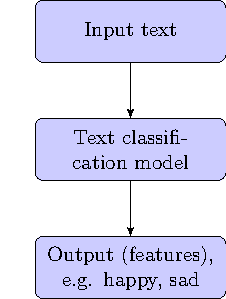
\includegraphics[width=2.5 in]{images/tcworkflow}
\caption{Text Classification Workflow}
\label{tcworkflow}
\end{figure}

The first step to classify text is to treat text as a bag of words \cite{Brilis2012}. Bag of words is a model in natural language processing that treats texts as unordered words, and the frequency of each word would be recorded. This process is usually conducted by tokenization, and followed by stemming and lemmatization. Stemming and lemmatization can delete the additional part of the word, remain only the stem part. For example, after stemming and lemmatization, the word "interesting" would become "interest". After stemming and lemmatization, stop words, which are words that have no actual meaning in a sentence, will be removed from the bag of words. An example of a stop word can be "and".

One way to classify texts is a Naive Bayes algorithm. Naive Bayes is based on Bayes’ probability theorem \cite{DBLP:journals/corr/Raschka14}. In Bayes’ probability theorem, for event A and B, the conditional probability of A given B is equation \eqref{eq:5}.

\begin{equation}
  P(A | B)=\frac{P(B | A) \cdot P(A)}{P(B)}
  \label{eq:5}
\end{equation}

Multinomial naive Bayes is one of the ways to use the Naive Bayes algorithm to classify texts. It uses the term frequency, $tf(t,d)$, where $t$ is term, and $d$ is the active document. Let $tf(t,d)$ be the frequency of term $t$ in document $d$, and $n_{d}$ be the total number of terms in document. As the equation \eqref{eq:6} shows.

\begin{equation}
  \text { term frequency }=\frac{t f(t, d)}{n_{d}}
  \label{eq:6}
\end{equation}

Spotify uses textual information from the internet to find key terms for music content. The terms will be used to build vectors for each song. A similar technique used in collaborative filtering will be applied to find similar content. This technique has a flaw that the textual information gets from the internet is too broad. It will be better if the information is from the comments under each song directly. That way, each song will have a direct correlation to the key terms. Except for comments, user search history could also be used as part of the text \cite{Bu2010}.

\subsection{Audio Metadata Modeling}

Audio metadata is the information for the audio files, it usually contains names for artist, album, title, genre, track number, and more \cite{audio2018}. After sampling the audio, more information can be included in audio metadata, for example, loudness, tempo, and more. This information can be used to predict potential music or human emotions. Tempo represents the speed of the audio, it is related to human emotions according to studies. Fast tempo and emotions like joy and fear have correlations, slow tempo and emotions like sadness and tenderness have correlations \cite{kamenetsky1997effect}.

Spotify has a database that contains the audio metadata. These aspects can be used to build vector representations. By applying a similar technique in collaborative filtering, similar content will be identified. Bogdanov et al. proposed a way of classifying music by using audio metadata \cite{bogdanov2013semantic}. They asked participants to choose their preferred music and categorized them based on their preferences. They then modeled the audio files and classified them. After that, they correlated the classified features with predefined categories. By using this model, they can suggest songs based on audio metadata.

\section{Content-Based Music Information Retrieval}

Besides collaborative filtering, content-based music information retrieval is another effective way of recommending. This method collects information that describes the music, and use the information to suggest new content. Audio metadata can be one of the sources for the information.

One application is to collect and classify audio signal features, then apply them to match based on different situations. In general, there are two ways of matching, which are query by example, and query by humming \cite{Kaminskas2012}. Query by example means getting the audio signal as input and return music metadata as output. This query method works on the specific music track, but not the variation tracks, for example, a cover version. Query by humming makes it up by getting melody as input and returns similar tracks. This application is more of a searching or matching algorithm. The limitation of this recommendation method is as I mentioned previously, lack of novelty \cite{Kaminskas2012}. It only expands on user saved songs, and it cannot predict user situation.

The other application is to combine the information which describes the music with user preferences. The user preference does not mean the user ratings, content-based music recommendation does not rely on user ratings \cite{Celma2010}. However, categorizing music content based on descriptive information requires experts of the fields to set rules. A similarity check is also required for the content-based suggestion. The way of calculating the similarity between two items is through calculating their distance. The common ways of calculating such distance are Euclidean distance \eqref{eq:7}, Manhattan distance \eqref{eq:8}, vector cosine distance\eqref{eq:1}, Mahalanobis distance \eqref{eq:9}, and Chebyshev distance \eqref{eq:10}.

\begin{equation}
  d=|x-y|=\sqrt{\sum_{i=1}^{n}\left|x_{i}-y_{i}\right|^{2}}
  \label{eq:7}
\end{equation}

Euclidean distance measures the straight line between two points in N-dimensional space \cite{euclidean}.

\begin{equation}
  d(x, y)=\sum_{i=1}^{n}\left|x_{i}-y_{i}\right|
  \label{eq:8}
\end{equation}

Manhattan distance is also a measurement of the straight line between two points in N-dimensional space. Just imagine the street blocks in Manhattan, there two paths from one intersection to the other one. However, the true distance between them is a straight line cut through the buildings \cite{craw1970}.

\begin{equation}
  d(x, y)=\sqrt{(x-y)^{T} S^{-1}(x-y)}
  \label{eq:9}
\end{equation}

Mahalanobis distance is a measurement of the straight line distance between two points in N-dimensional space. Mahalanobis distance handles better with correlated points($\ge2$). In situations that there are more than 2 points that are correlated, the axes of the points are no longer orthogonal, and they cannot be plotted in 3-dimensional space \cite{stephanie2018}.

\begin{equation}
  d(x, y)=\max _{i=1 . . . n}\left|x_{i}-y_{i}\right|
  \label{eq:10}
\end{equation}

Chebyshev distance, also called maximum value distance, is similar to Euclidean distance and Manhattan distance. It calculates the straight line distance based on point coordinates.

There are limitations for this application when new users entered the system, they can't get the right suggestion because the system needs time to adjust to the user preferences. This situation is also called the cold-start problem \cite{Celma2010}. Another issue is feature extraction. It is hard to extract high-level descriptions such as mood. These high-level descriptions are very important in accurate and personalized recommendations.

\section{Contextual Music Retrieval}

Contextual music information is any information, other than music content information, that describes the music content itself. Contextual music suggestion means to recommend music based on the user's actual situation, for example, emotional state. This method takes three sources of information, environment-related context, user-related context, and multimedia context \cite{Kaminskas2012}. Environment-related information can be the season, temperature, time, and weather because all these contexts can influence human emotions. User-related information can be user activities, such as exercising and driving, user profiles, such as social network statements, and emotional state. Multimedia can be text and image relevant to the music. This information can be used to profile and predict the user's actual situation. After the necessary information is gathered, similarity predicts, classification, and other techniques can be used to predict user preferences.

Another way of achieving contextual music retrieval is proposed by B. Han et al \cite{Han2010}. They proposed an emotion state transition model which models music-evoked human emotions, and content-based music recommendation ontology to profile user preference and context. The system provides music by mapping high-dimensional music features with the emotion state transition model. According to the paper, this method achieved 67.54\% overall accuracy. The limitation of this method is that it needs a large amount of data, and the human emotional state can be changed based on the social environment. Once the social context is changed, more data would be required to get higher accuracy.

Recommendation based on contextual music retrieval is still new, and it has great potential to contribute to the music recommendation system.


%\numberedchapter{Method Of Approach}
\chapter{Method of Approach} 
\label{ch:method}

This chapter should answer the ``how'' question - how did you complete your project, including the overall design of your study, details of the algorithms and tools you have used, etc.  
 Use technical diagrams, equations, algorithms, and paragraphs of text to
describe the research that you have completed. Be sure to number all figures and tables and to explicitly refer to them in your text.


%\numberedchapter{Experimental Results}
\chapter{Experimental Results}
\label{ch:experiments}

% This chapter should describe your experimental set up and evaluation. It should also produce and describe the results of your study. Possible section titles are given below.

\section{Experimental Design}

\subsection{Program Tests}



\subsection{User Tests}

\subsubsection{Institutional Review Board}

The form of user tests are surveys. To conduct the user servey, the designed survey
have to be approved by Allegheny College Institutional Review Board (IRB). Institutional
Review Board is an organization that reviews and supervises experiments to make
sure the human rights of participants do not get hurt \cite{irb}. Before the application
starts, experimentors have to finish a Collaborative Institutional Training Initiative
(CITI Program) \cite{citi}. The program required by the Allegheny College Institutional
Review Board is Social & Behavioral Research. To get approved by the IRB, a proposal
first have to be submitted. The proposal contains review questions to help experiment
designer and organizers to identify the type of experiment because certain types
of experiment can get exemption or expedition. The questions are, for example,
does the experiment involves human, does the experiment involves individuals under
the age of 18. This experiment required exempted review. Other than the review
type, a brief introduction, procedure, and walk-through should be included.

\subsubsection{Description and Rationale of Project}

The description and rationale of project included in the Institutional Review
Board proposal are as follows:

This develops a novel software system to recommend songs to users. The mainstream
music service providers utilize user browsing and listening history along with
comparison of the user’s playlist to that of other users with similar habits to
recommend music to users.  In this project, instead of standard data, our system
uses machine learning to identify the user's current emotion by asking a user to
enter a text that contains some indication of their current emotions and feelings.
The text entered by the user can be their diary, a transcribed conversation, or
a script from a show that their current emotional state relates to. Using this
text, our system then learns about the users’ current emotional state and uses
that information to predict desired musical themes and songs to the user. The
purpose of the user study is to verify the efficiency of this software system,
where the participants are asked to provide a short body of text, and following
the review of the recommended song list they are invited to provide feedback on
the outcome they received.

\subsubsection{Methods and Procedures}

The methods and procedures of the experiment included in the Institutional Review
Board proposal are as follows:

The participation for this study will be advertised on My Allegheny, and via
departmental announcements (posters, club emails, Slack channel). The individuals
who agree to participate in the study will be emailed a link to the website on
which our system operates. Once on the landing page of the website, the participants
will be provided information about the experiment and they will be informed that
their consent is received if they proceed with the next steps of the study.  In
the next steps, the participants will create an account in our system and then
log in to their unique account. The walk-through section contains detailed sequence
of steps that the participants will be involved in and the pages on our website
that they will be directed to.

The website will be hosted on a private cloud-based server (Amazon Cloud Server, AWS).
The IP addresses and other information that could associate with the participants
will be deleted before analyzing the data. The data will be kept for four years
for possible further study, and it will be deleted after four years. AWS’s data
centers and network architecture is designed to protect information, identities
and applications stored in their cloud by following core security and compliance
requirements. The information required for the registration will be the username
and password. After logging in, the participants will be asked to follow the
instructions on the website and provide a body of text that reflects their emotions
on three different days. The following instructions will be provided:

\begin{displayquote}
  Please choose three days of this week, and for each day:

  \textbf{Option 1:} Provide more than a paragraph of text in any form (e.g. diary)
  that best describes your emotions or experiences on that day.

  \textbf{Option 2:} Provide more than a paragraph of a conversational or summarization
  text (e.g. TV scripts or TV scene summarization) that describes an emotional scene.

  Please provide a descriptive title to each body of text that you enter.
\end{displayquote}

After receiving the bodies of text from the user, our system will automatically
provide a list of recommended songs. After getting the recommended music playlist,
participants will be invited to participate in the survey by answering the following
three questions:

\begin{displayquote}
  \begin{enumerate}
    \item Describe the body of text that you provided. What emotions did you want
    to express in this text?
    \item Please choose the best description for the recommended playlist.
    \begin{enumerate}
      \item This playlist has nothing to do with my text
      \item I can see a rare relation to my text
      \item This playlist is acceptable, but I do not have a strong emotional
      connection to it
      \item I have a fair amount of an emotional connection to this playlist
      \item I have a strong emotional connection to this playlist
    \end{enumerate}
    \item If you feel an emotional connection to this playlist, why do you think
    the music is related to your provided text? If you do not feel a connection
    to this playlist, what do you think the playlist is missing?
  \end{enumerate}
\end{displayquote}

The goal of the questions in the survey above is to assess the efficiency of the
algorithm and the participants’ interpretation of their feelings. The answers will
be collected on the same website of our system and the answers will be connected
to specific user accounts. The user account is the only connection between the
answers and the provided bodies of text by the user. Again, all the user information,
including IP address, browser information, usernames, and passwords will be deleted
before the analysis of the collected data.

After the survey, the data will be analyzed using the responses in the user satisfaction
from question 2. Responses in the range from 1 to 3 will be marked as “need for
further analysis”. Question 1 and question 3 will be used to interpret the unsatisfied
playlist. The summary of the analyzed results will be reported in a senior thesis
document that will be stored on the cloud-based version-control system, called GitHub.
All participants who indicate an interest in receiving the results of the study
will be emailed a link to the GitHub page containing the senior thesis document.

The potential risks of this study is that the participants may spend a long time
writing texts. They  may also have to think about sad memories. If the participants
do not wish to proceed, they may quit any time during the process by pushing the
\emph{quit} button on the page.

\subsubsection{Walk-Through}

Participants will receive a link to begin their participation in this user study.
When participants click on the link, they will land on the “Information” page.

\subparagraph{Information Page}

After entering the website, users would see an information page that contains the
following message:

\begin{displayquote}
  \textbf{Project introduction:}

  This project develops a novel software system to recommend songs to users. The
  mainstream music service providers utilize user browsing and listening history
  along with comparison of the user’s playlist to that of other users with similar
  habits to recommend music to users. In this project, instead of standard data,
  our system uses machine learning to identify the user's current emotion by asking
  a user to enter a text that contains some indication of their current emotions
  and feelings. The text entered by the user can be their diary, a transcribed
  conversation, or a script from a show that their current emotional state relates
  to. Using this text, our system then learns about the users’ current emotional
  state and uses that information to predict desired musical themes and songs to
  the user. The purpose of the user study is to verify the efficiency of this
  software system, where the participants are asked to provide a short body of
  text, and following the review of the recommended song list, participants are
  invited to provide feedback on the outcome they received.

  \textbf{Data usage:}

  This research is anonymous, the IP addresses and other personal information
  that could be associated with the participants will be deleted before analyzing
  the data. The data will be kept securely on Amazon Web Services for four years
  for possible further study, and they will be deleted after four years. The
  information required for the registration is the username and password. If you
  wish to receive a copy of the results of the study, please answer “yes” in the
  google survey form under the result disclosure section. A copy of the report of
  the study in the form of the senior thesis project document will be sent to you
  upon the completion of the analysis.

  \textbf{Exiting the study:}

  The potential risks of this study is that the participants may spend a long
  time writing texts. They  may also have to think about sad memories. If you
  feel uncomfortable in any of the sections during the process, you can click the
  quit button. If you decide not to stop the participation, you can email the
  principal investigator of the project at \emph{liux2@allegheny.edu} to request
  immediate deletion of any data you have created.

  \textbf{Compensation:}

  All participants will have the opportunity to join a drawing for a chance to
  win a \$20 Amazon gift card. Please answer “yes” in the google survey form under
  the lottery section if you want your name to be entered into the drawing. All
  participants will receive a notification of the results of the drawing.

  \textbf{Contact information:}

  If you have any questions, please contact us.

  \textbf{Xingbang Liu:}

  \textbf{Phone:} (814)-795-0122

  \textbf{E-mail:} liux2@allegheny.edu

  \textbf{Professor Janyl Jumadinova:}

  \textbf{E-mail:} jjumadinova@allegheny.edu

  If you consent to the participation in this study, please continue with the
  next step.
\end{displayquote}

After participants log in, they will be taken to the “Text Entering” page.

\subparagraph{Text Entering Page}

After participants enter their text according to the instruction, they will be
directed to the “Result” page containing their recommended playlist, below which
information about the survey will be included.

\subparagraph{Result Page}

After listening to the songs recommended, users can proceed to the servey.

\begin{displayquote}
  \textbf{Survey 1:} Please click on this link for the survey to provide feedback
  on your recommended playlist.

  \textbf{Survey 2:} Please click on this link to indicate your interest in receiving
  the results of this study and your interest in entering the drawing.
\end{displayquote}

\section{Evaluation}

\section{Threats to Validity}


%\numberedchapter{Conclusion}
\chapter{Discussion and Future Work}  
\label{ch:conclusion}

This is the conclusion. You might want to leave it unnumbered, as it is now. If you want to number it, treat it like any other chapter.

This chapter usually contains the following items, although not
necessarily in this order or sectioned this way in particular.

\section{Summary of Results}
A discussion of the significance of the results
and a review of claims and contributions.

\section{Future Work}

\section{Conclusion}


 
%----------------------------------------------------------------------------------------
%	BIBLIOGRAPHY
%----------------------------------------------------------------------------------------

\addtocontents{toc}{\vspace{2em}} % Add a gap in the Contents, for aesthetics
\unnumberedchapter{Bibliography} % Title of the unnumbered chapter
\bibliography{preamble/bibliography} % The references information are stored in the file named "bibliography.bib"


\end{document}  